\documentclass[Nike]{tuberlinbeamer}

\usepackage[ngerman]{babel}  % 'babel' muss geladen werden
\usepackage[utf8]{inputenc}  % optional, aber empfehlenswert
\usepackage[T1]{fontenc}

\usepackage{svg}
\usepackage[export]{adjustbox}
\usepackage{amssymb}

% Die ueblichen Angaben
\title{PAVOOC - Prediction and visualization of on- and off-targets for CRISPR}
\subtitle{Master thesis}
\author[Moritz Schäfer]{Moritz Schäfer}
\institute{Technische Universität Berlin \& Bayer Pharma}

% Eigenes Logo einfuegen:
\renewcommand{\pathtomylogo}{meinlogo}

\begin{document}

\begin{frame}
\maketitle
\end{frame}


% \begin{frame}
% \frametitle{Outline}
% \tableofcontents
% \end{frame}

\section{Background}
\begin{frame}{Background}
  \begin{figure}
    \hspace*{0.2in}
    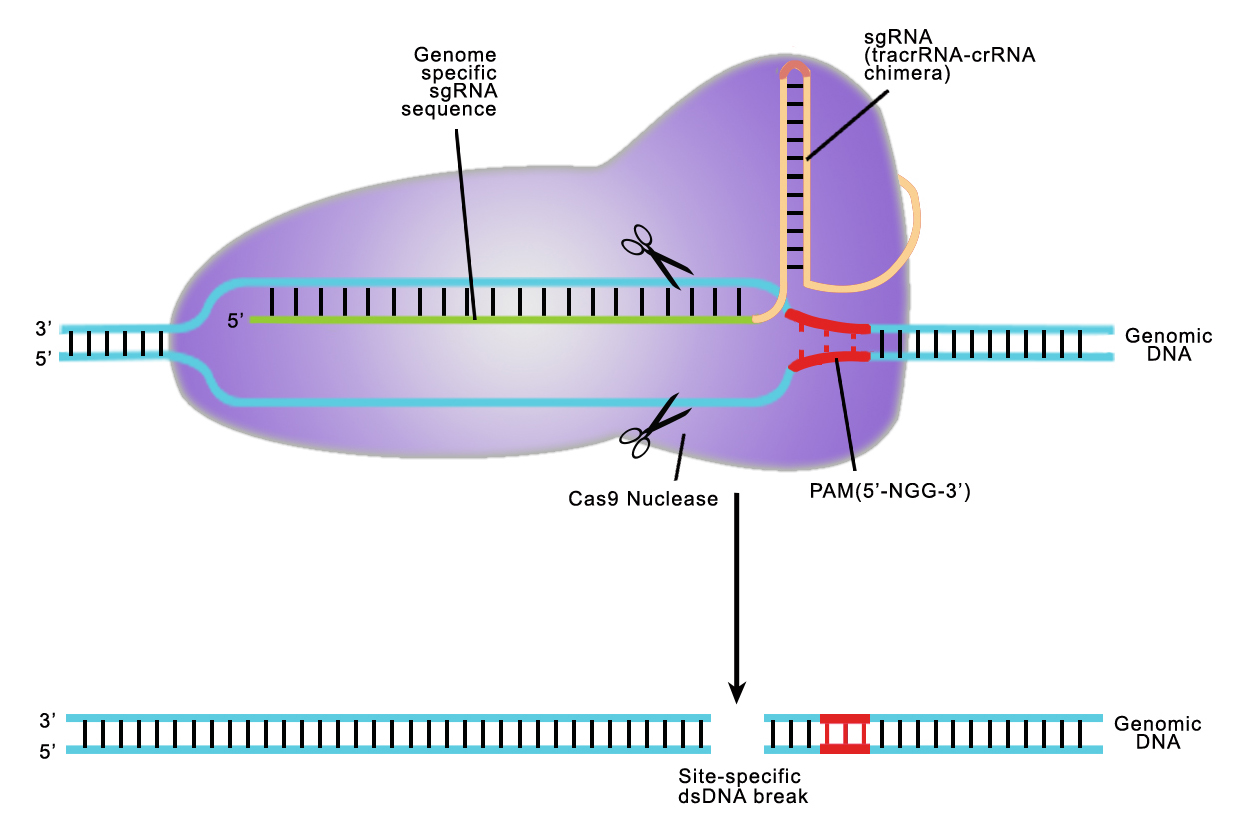
\includegraphics[width=0.57\linewidth,left]{Doudna-art-crop.jpg}
  \end{figure}
  \begin{itemize}
    \item Knockout experiments used in drug target validation
    \item Sequence (partially) determines efficacy
  \end{itemize}
\end{frame}

\section{Problem}

\begin{frame}
  \frametitle{Problem}
  \begin{itemize}
    % \item Many tedious and incomplete guide design tools \\
    %   \texttt{./guidesearch | ./convert\_output.sh | ./score\_guides > output.csv}
    \item Guide prediction scores still vary in performance
    \pause
    \item A lot of manual labor for guide selection \\
      \includegraphics[width=0.7\linewidth,left]{xlswork.png}
    \pause
    \item Non-frame-shift indels cannot be circumvented
      \includegraphics[width=0.6\linewidth,left]{nonframeshift.png}
    \pause
    \item Cancer cellline data affects certain guides
      \includegraphics[width=0.3\linewidth,left]{guide_snp.png}
  \end{itemize}
\end{frame}

\section{Solution}

\begin{frame}{Solution}
  \begin{itemize}
    \item Cutting-edge guide efficacy scoring
    \item All-in-one guide design tool
      % So it is easy to use for pure biologists only
    \item Functional domain-aware
    \item Incorporate cancer cellline data
  \end{itemize}
\end{frame}

% So what I wanna show you here is an overview of the solution I built.
% LIVEDEMO HERE
\begin{frame}{Live Demo}
  Live Demo
\end{frame}{Live Demo}

% As I told before, one large part of my work was to improve the guide efficacy scoring.
\subsection{Guide efficacy prediction}

\begin{frame}{Guide efficacy prediction -- Dataset}
\begin{table}[]
    \centering
    \begin{tabular}{cc}
        \textbf{Guide} & \textbf{Measured efficacy} \\ \hline
\texttt{GTAGGGGTCCGTACTCAGCAAGG} & 0.86 \\
\texttt{ACACTGCCGAGCGATGAGGATGG} & 0.42 \\
\texttt{AAGGTGAAGGAGGATGCGGCGGG} & 0.53 \\
\texttt{GAAAAGATAGGTCACTGACCCGG} & 0.12 \\
\texttt{GCAAGTCACTGAGTGCAGAACGG} & 0.73 \\
\texttt{GCATTGGTAAGCGCACAGGAAGG} & 0.70 \\
\texttt{AAGACTGGCGCATGGTCCACTGG} & 0.57 \\
\texttt{...} & ... \\
    \end{tabular}
\end{table}
\begin{itemize}
  \item 5310 data rows
  \item Efficacy relates to cell proliferation after CRISPR application
\end{itemize}
\begin{flushright}
  \tiny
  ``Optimized sgRNA design to maximize activity and minimize off-target effects of CRISPR-Cas9'', 2016, John G. Doench et al.\
\end{flushright}
\end{frame}

\begin{frame}{Guide efficacy prediction -- 1st gen.}
  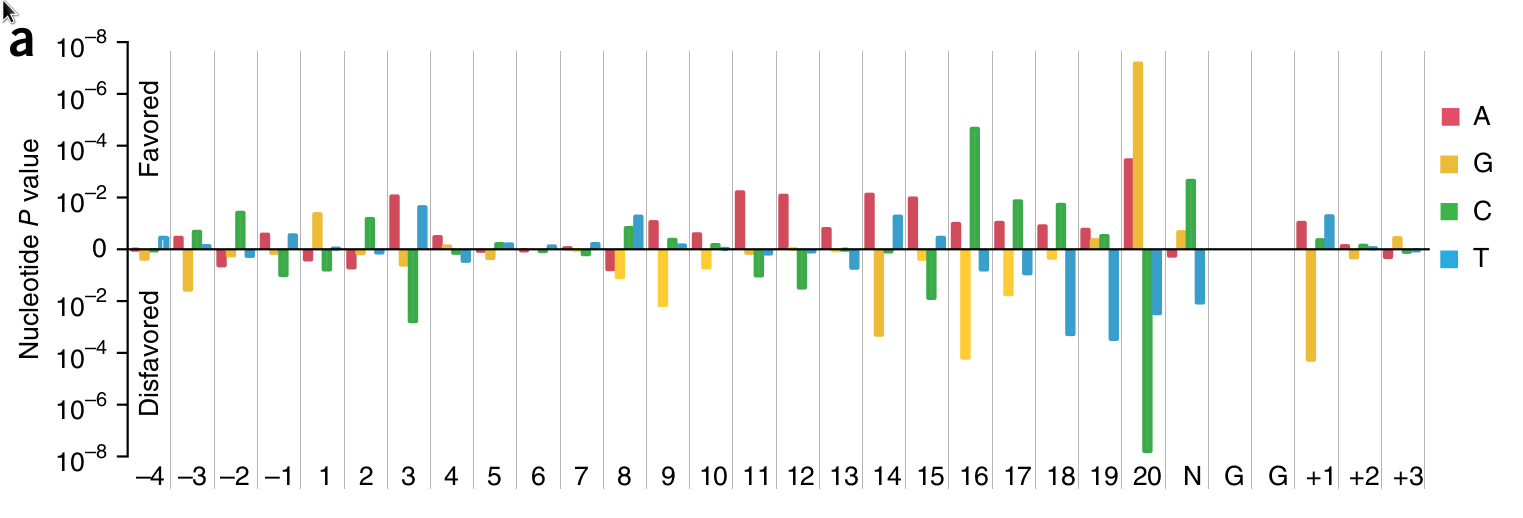
\includegraphics[width=\linewidth]{./nucleotide_table.png}
  \begin{flushright}
    \tiny
    ``Rational design of highly active sgRNAs for CRISPR-Cas9–mediated gene inactivation'', 2014, John G. Doench et al.\
  \end{flushright}
  %What early publications noticed, is that the effectiveness of a guide to a great extend depends on the sequence of nucleotides
\end{frame}

\begin{frame}{Guide efficacy prediction -- 2nd gen.}
  % Later publications then identified COMBINED adjacent nucleotides as predictive features
  Pairwise nucleotide features

  \pause
  \huge ACTATCTATCGTACGA{\color{red}TT}GA \\
    \pause
  ACTATCTATCGTACGAC{\color{red}AA}G
    \begin{flushright}
      \tiny
      ``Optimized sgRNA design to maximize activity and minimize off-target effects of CRISPR-Cas9'', 2016, John G. Doench et al.\
    \end{flushright}
    \pause
  \center
  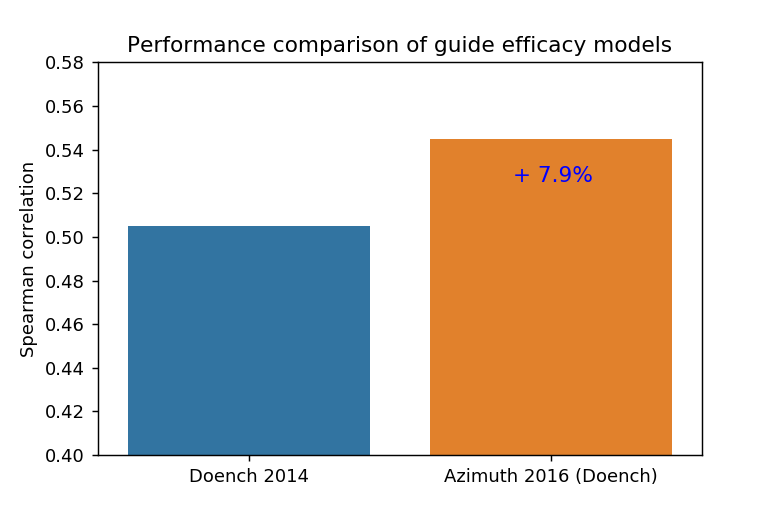
\includegraphics[width=0.5\linewidth]{./model_comparison1.png}
\end{frame}

% Unfortunately, the models they used to identify these combinations only allowed for investigating pairs of nucleotides, though we don't know if three four or more adjacent nucleotides do interact in a way that they influence Cas9 binding.

% To be able to identify such larger combinations, I use a tool called

\begin{frame}{Convolutional neural networks}
  % The motivation behind Convolutional neural networks
  Aim: Find spatial patterns
  % This is usually used for image recognition and makes finding edges and shapes very efficient
  \pause
  % So if you have this filter here, and convolute it over the image, comparing it with all possible areas in the picture, it will signal a positive result on this area. This makes it a good filter for detecting parts of noses.
  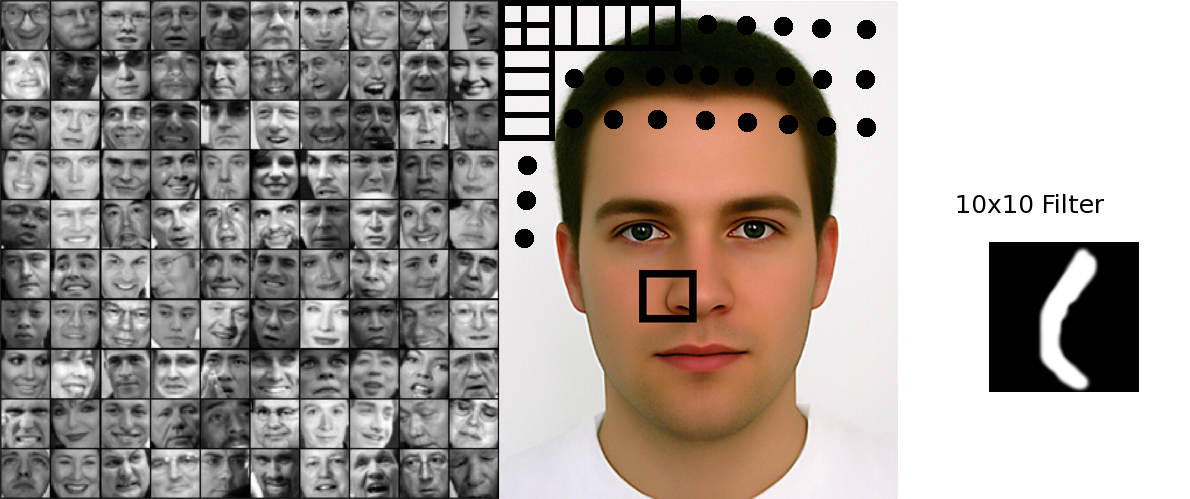
\includegraphics[width=0.7\linewidth]{./nosefilter.png}
\end{frame}
%Now the cool thing is, that a convolutional neural networks learns these shapes on its own just be looking at a ton of images. You tell it to classify noses, it will learn filters to detect nose specific shapes.

% Now the same thing also works with sequences:
\begin{frame}{Convolutional neural networks}
  % A 4 character long text filter could look like this
  \huge[A C A A]
  \pause
  % Now if we've got 1000 guide RNAs
  \vspace{0.7cm}
  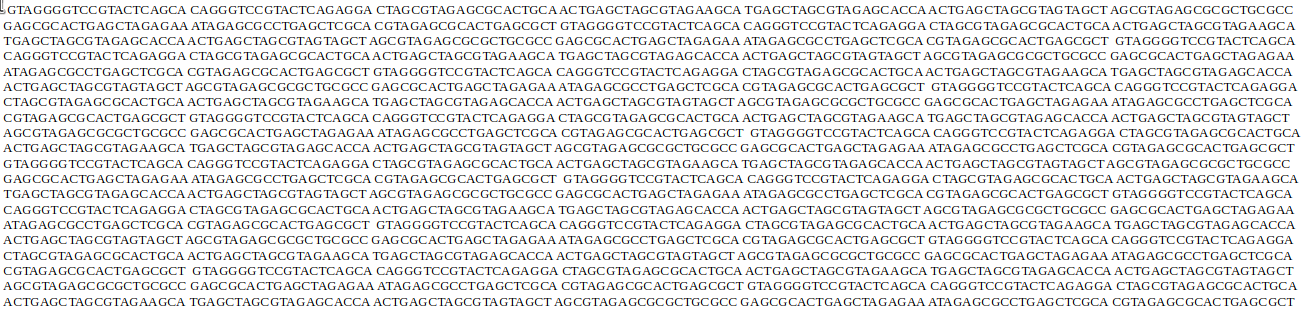
\includegraphics[width=\textwidth]{./manyguides.png}
\end{frame}

\begin{frame}{Convolutional neural networks}
  % Ok that's probably a bit too much
  % Let's say we've got 10 guide RNAs which performed really well in a CRISPR experiment. So they all provoked a Double strand break at their target position.
  Well performing guides: \\
  {\large
    GTAGGGGTCCGTACTCAGCA \\
    CAGGGTCCGTACTCAGAGGA \\
    CTAGCGTAGAGCGCACTGCA \\
    ACTGAGCTAGCGTAGAAGCA \\
    TGAGCTAGCGTAGAGCACCA \\
    ACTGAGCTAGCGTAGTAGCT \\
    AGCGTAGAGCGCGCTGCGCC \\
    GAGCGCACTGAGCTAGAGAA \\
    ATAGAGCGCCTGAGCTCGCA \\
    CGTAGAGCGCACTGAGAGCT \\
  }
  % now if you look closely at the last four nucleotides, you notice that they are very similar. A convolutional neural network can recognize this similarity and rerember it with help of a filter.
\end{frame}

\begin{frame}{Convolutional neural networks}
  Well performing guides: \\
  {\large
    AGCA \\
    AGGA \\
    TGCA \\
    AGCA \\
    ACCA \\
    AGCT \\
    CGCC \\
    AGAA \\
    CGCA \\
    AGCT \\
  }
  \pause
  Learned filter: {[A G C A]}
  % And this is exactly what we want: This filter now helps the neural network to recognize well performing guides
\end{frame}

\begin{frame}{Model architecture}
  \begin{figure}
    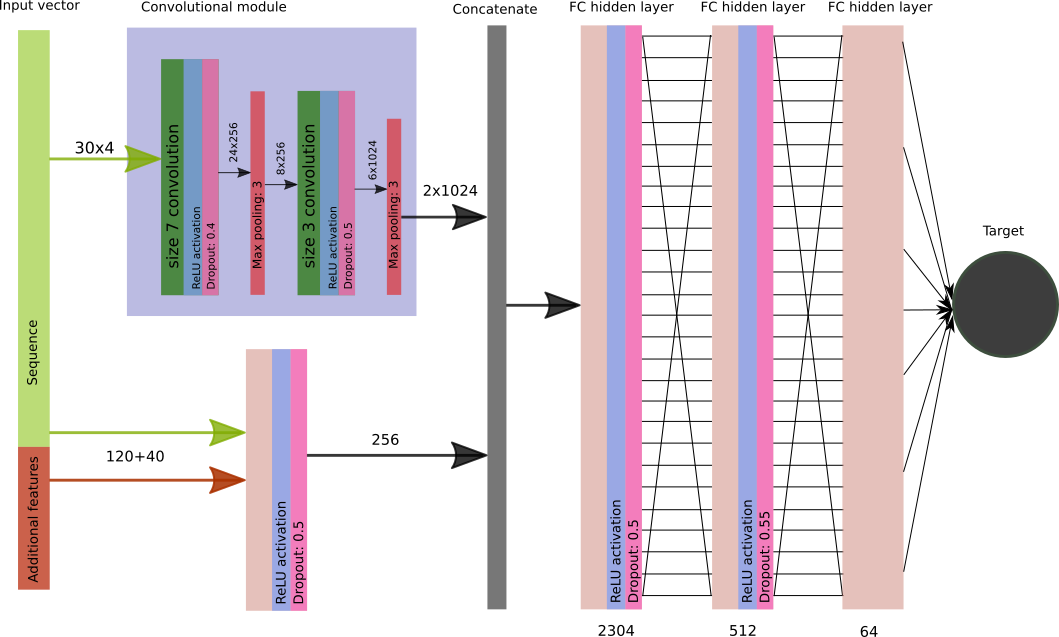
\includegraphics[width=0.65\linewidth]{CNN38_layout.png}
  \end{figure}

\end{frame}

\begin{frame}{Model architecture}
  \begin{figure}
    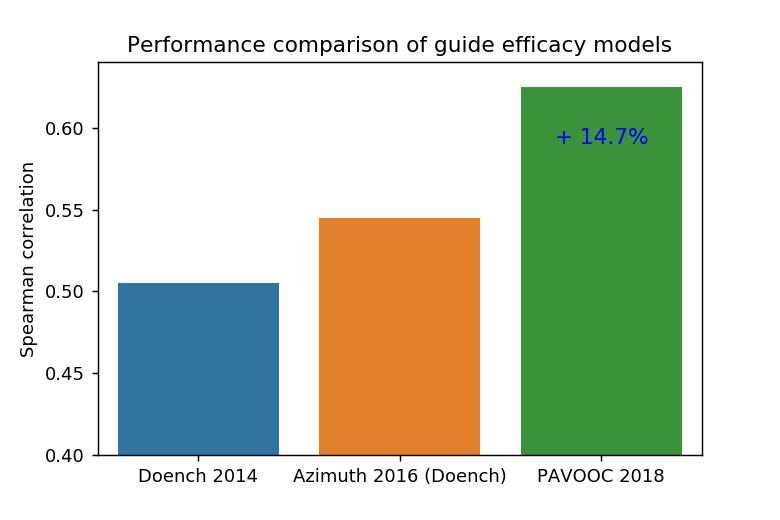
\includegraphics[width=0.65\linewidth]{model_comparison2.png}
  \end{figure}

  Conclusion: Deep Learning improves guide efficacy prediction
\end{frame}

% To build the web application, I first developed a data processing pipeline that gathers various relevant data sources, preprocesses them and stores them in an easy to access format in a database. From this data I also generated the BED files being using in the Sequence Browser.
\begin{frame}{Architecture}
  \begin{figure}
    \centering
    \includegraphics[width=0.65\linewidth]{architecture.png}
  \end{figure}
\end{frame}

\begin{frame}{Acknowledgements}
  \begin{itemize}
    \item Dr.\ Andreas Steffen (supervisor at Bayer)
    \item Prof.\ Manfred Opper (supervisor at TU Berlin)
    \item Dr.\ Djork-Arne Clevert (machine learning scientist at Bayer)
    \item Robin Winter (PhD student at Bayer)
    \item Bayer Pharma AG
  \end{itemize}

\end{frame}
\end{document}
